\documentclass[a4paper,10pt]{article}
\usepackage{trymtex}
\usepackage[backend=biber,style=alphabetic]{biblatex}
\usetikzlibrary{arrows.meta,calc,positioning}

\addbibresource{references.bib}

\begin{document}
\begin{titlepage}
    \newcommand{\HRule}{\rule{\linewidth}{0.5mm}}
    \begin{tikzpicture}[remember picture, overlay]
      % NTNU logo
      \node[anchor=north west, xshift=1.0cm, yshift=-1.0cm] at (current page.north west) {
        \includegraphics[width=2.0cm]{figures/ntnu_logo_liten.png}
      };
    \end{tikzpicture}
  
    \center

    % Course code & title
    {\color{ntnu-blue}\sffamily\large TMA4212 \par}
    {\sffamily\Large Numerical Solution of Differential Equations by Difference Methods \par}
    
    \HRule
    \vspace{1.5cm}
  
    % Assignment title
    {\large\sffamily\bfseries Project 2\par}
    \vspace{0.3cm}
    {\Large\sffamily\textit{Solving the Poisson equation, and an Optimal Control Problem\\ using the Finite Element Method}\par}
  
    \vspace{0.5cm}
    \HRule
  
    \vfill
  
    % Author info
    \begin{minipage}{0.6\textwidth}
      \begin{flushleft}
        \large
        \textbf{Authors:}\\
        Haugen, Tor Ludvig Løvold \\
        Sæther, Trym\\ 
      \end{flushleft}
    \end{minipage}%
    \begin{minipage}{0.4\textwidth}
      \begin{flushright}
        \large
        \textbf{Semester:}\\
        Spring 2025
      \end{flushright}
    \end{minipage}
  
    % University logo/name
    \begin{center}
      {\color{ntnu-blue}\sffamily\Large Norwegian University of Science and Technology}\\
      \vspace{0.3cm}
      {\sffamily\large Department of Mathematical Sciences}
  
      \vspace{0.5cm}
      {\large\today}
    \end{center}
  
    \vspace{1cm}
  \end{titlepage}
  
  
  
\clearpage

\section[Quadratic FEM for Poisson]{Solving a 1D Poisson Equation with Quadratic Finite Elements}
\subsection{Variational Formulation and Galerkin Method}
The Poisson boundary-value problem to solve is: find \(u(x)\) on \(\Omega=(0,1)\) such that
\[
-u^{\prime\prime}(x) = f(x), \quad u(0)=u(1)=0 \text{ (Dirichlet BC)}.
\]
In variational (weak) form, this is formulated as: find \(u \in V\) such that
\[
a(u,v) = F(v) \quad \forall v \in V,
\]
where \(V = H^1_0(\Omega)\) (functions vanishing at the boundaries).
The bilinear form and linear functional are
\[
a(u,v) = \int_0^1 u'(x)\,v'(x)\,dx, \qquad F(v) = \int_0^1 f(x)\,v(x)\,dx.
\]
This weak formulation arises from multiplying the PDE by a test function \(v\), integrating by parts, and applying the zero boundary conditions.

The Galerkin finite element method restricts this infinite-dimensional problem to a finite-dimensional subspace \(V_h \subset V\). 
We seek an approximate solution \(u_h \in V_h\) such that
\[
a(u_h, v) = F(v) \quad \forall v \in V_h.
\]
This means \(u_h\) satisfies the same variational equation but only for test functions \(v\) in the finite element space \(V_h\). By construction of \(V_h\), this yields a symmetric linear system of equations for the coefficients of \(u_h\).

\subsection{Finite Element Space and Quadratic Basis Functions}
We use a \emph{second-degree Lagrange finite element space \(\mathbb{P}_2\)} for the approximation.
Specifically, let \(\mathcal{T}_h\) be a partition of \([0,1]\) into \(M\) elements, and define
\[
	X_h^2 = \{ v \in C^0([0,1]) : v|_{K} \in \mathbb{P}_2,\ \forall K \in T_h\},
\]
i.e. \(X_h^2\) consists of continuous piecewise-polynomial functions of degree \(\le 2\) on each element.

We then take \(V_h = X_h^2 \cap H^1_0(\Omega)\) , enforcing \(v(0)=v(1)=0\) (the Dirichlet boundary conditions) so that the boundary conditions are built into the space.
In this setup, each element has three local nodes and hence three local basis shape functions.

Globally (with \(M\) elements and two new nodes per element, but sharing at interfaces), the dimension of \(V_h\) is \(2M-1\) (for \(M\) elements, there are \(2M+1\) total nodes including boundaries, and we remove the 2 boundary nodes because of \(H^1_0\)).

\begin{example}{Equidistant partition}{equidistant_poisson}
	An equidistant partition with \(M=5\) elements would have \(11\) total basis functions (including the boundary nodes, which are fixed to zero).
\end{example}

\subsection*{Mesh and nodes}
We label the nodes in a convenient way for quadratic elements.
Suppose we choose partition points \(0 = x_0 < x_2 < x_4 < \cdots < x_{2M} = 1\) for the element endpoints.

Each element \(K_k\) spans from \(x_{2k}\) to \(x_{2k+2}\), and we introduce the midpoint \(x_{2k+1} = x_{2k} + \frac{1}{2}(x_{2k+2}-x_{2k})\) as the middle node.
Thus each element \(K_k = [x_{2k},\,x_{2k+2}]\) has three nodes: \(\{x_{2k}, x_{2k+1}, x_{2k+2}\}\) (left endpoint, midpoint, right endpoint).

Globally, the set of all nodes is \(\{x_0, x_1, ..., x_{2M}\}\) with \(x_0=0\) and \(x_{2M}=1\).
Interior \emph{even-indexed} nodes (\(x_2, x_4, ..., x_{2M-2}\)) are shared between two adjacent elements, ensuring continuity, while \textit{odd-indexed} nodes (\(x_1, x_3, ..., x_{2M-1}\)) are midpoints unique to a single element.

\subsection*{Basis functions}
On each element, we use \emph{quadratic Lagrange shape functions} associated with the local nodes.
We first define shape functions \(\{\Psi_0, \Psi_1,\Psi_2\}\) on the \emph{reference element} \(\hat K = [0,1]\), taking the local reference nodes as \(\xi_i = \{0, \frac{1}{2}, 1\}\) (the left endpoint, midpoint, and right endpoint).
We choose \(\Psi_\alpha(\xi_\beta) = \delta_{\alpha\beta}\), meaning \(\Psi_0(0)=1, \Psi_0(0.5)=0, \Psi_0(1)=0\), etc.

These are the standard quadratic Lagrange basis on \([0,1]\):
\begin{align*}
	\Psi_0(\xi) & = 2\xi^2 - 3\xi + 1, \\
	\Psi_1(\xi) & = -4\xi^2 + 4\xi,    \\
	\Psi_2(\xi) & = 2\xi^2 - \xi.
\end{align*}


Each \(\Psi_i\) is a polynomial of degree 2 on \([0,1]\).
They satisfy \(\Psi_0(0)=1\), \(\Psi_1(0.5)=1\), \(\Psi_2(1)=1\), and all other combinations are zero, giving the Kronecker delta property.
The figure below illustrates these reference shape functions on \([0,1]\) and their values at the nodes:

\emph{Quadratic Lagrange shape functions} on the reference interval \([0,1]\). Each basis function \(\Psi_i(\xi)\) is 1 at its node and 0 at the other nodes. They form a \(C^0\) quadratic basis on one element.
\begin{figure}[H]
	\centering
	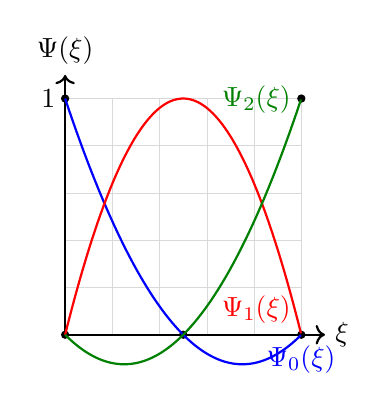
\begin{tikzpicture}[scale=3]
		% Grid
		\draw[very thin,color=gray!30] (0,0) grid[step=0.2] (1,1);
		\draw[->,thick] (0,0) -- (1.1,0) node[right] {\(\xi\)};
		\draw[->,thick] (0,0) -- (0,1.1) node[above] {\(\Psi(\xi)\)};

		% Reference points
		\fill (0,1) circle (0.5pt) node[left] {1};
		\fill (0.5,0) circle (0.5pt);
		\fill (1,0) circle (0.5pt);
		\fill (0,0) circle (0.5pt);
		\fill (1,1) circle (0.5pt);

		% Shape functions
		\draw[thick,blue,domain=0:1,samples=100] plot (\x,{2*\x*\x - 3*\x + 1})
		node[below] {\(\Psi_0(\xi)\)};
		\draw[thick,red,domain=0:1,samples=100] plot (\x,{-4*\x*\x + 4*\x})
		node[above left] {\(\Psi_1(\xi)\)};
		\draw[thick,green!50!black,domain=0:1,samples=100] plot (\x,{2*\x*\x - \x})
		node[left] {\(\Psi_2(\xi)\)};
	\end{tikzpicture}
	\caption{Quadratic Lagrange shape functions on the reference interval \([0,1]\).}
	\label{fig:quadratic-shape-functions}
\end{figure}

To get basis functions on a physical element \(K_k = [x_{2k}, x_{2k+2}]\), we use an \emph{affine mapping} \(\Phi_{K_k}: \hat K \to K_k\).
One convenient mapping is linear:
\[
	\Phi_{K_k}(\xi) = x_{2k} + \xi\, (x_{2k+2}-x_{2k}) \implies
	\begin{cases}
		\Phi_{K_k}(\xi=0) = x_{2k},     \\
		\Phi_{K_k}(\xi=0.5) = x_{2k+1}, \\
		\Phi_{K_k}(\xi=1) = x_{2k+2}.
	\end{cases}
\]
which sends \(\xi=\{0,0.5,1\}\) to \(\{x_{2k}, x_{2k+1}, x_{2k+2}\}\) respectively.

The local shape functions \(\phi_{k,\alpha}(x)\) on \(K_k\) are then defined by:
\[
	\phi_{k,\alpha}(x) = \Psi_\alpha(\xi), \quad \xi = \Phi_{K_k}^{-1}(x) = \frac{x-x_{2k}}{h_k}
\]
\[
	\phi_{k,\alpha}(x) = \Psi_\alpha\left(\frac{x-x_{2k}}{h_k}\right), \quad h_k = x_{2k+2}-x_{2k}.
\]
Because of the linear map, these \(\phi_{k,\alpha}(x)\) are still in \(\mathbb{P}_2\), just stretched or compressed to the element size.
Each local \(\phi_{k,\alpha}\) is supported only on element \(K_k\) and satisfies \(\phi_{k,\alpha}(x_{2k+\alpha})=1\) and \(\phi_{k,\alpha}(x) =0\) at the other two nodes of \(K_k\).

\subsection*{Global basis assembly}
The global basis functions \(\{\varphi_j(x)\}_{j=0}^{2M}\) are constructed from the local shapes by identifying them at shared nodes.
In practice, we label each global basis \(\varphi_j\) to correspond to node \(x_j\).
For example, \(\varphi_2(x)\) is the basis associated with the node \(x_2\), which is an endpoint of element \(K_1\) and \(K_0\);
\(\varphi_2\) is composed of the piece of \(\phi_{0,2}\) on \(K_0\) (which equals 1 at \(x_2\)) and the piece of \(\phi_{1,0}\) on \(K_1\), ensuring \(\varphi_2\) is continuous and piecewise quadratic.
Each interior node corresponds to a unique global basis function that may span one or two adjacent elements.

By construction, \(\varphi_i(x_j) = \delta_{ij}\), and any \(v_h \in V_h\) can be expanded as:
\[
	v_h(x) = \sum_{j \in \mathcal{N}_{int}} v_j\, \varphi_j(x),
\]
where the sum runs over all interior (free) nodes.

The boundary nodes \(x_0\) and \(x_{2M}\) are excluded in \(V_h\) because those basis functions would lie outside \(H^1_0\) (they would equal 1 at the boundary).
Thus we have \(2M-1\) basis functions for \(V_h\).

\subsection*{Assembly of Stiffness Matrix and Load Vector}
Using the Galerkin condition, we derive a linear system for the coefficients of \(u_h\).
Let \(\{ \varphi_j \}_{j=1}^{2M-1} \) be the global basis for \(V_h\).

We seek:
\[
	u_h(x) = \sum_{j=1}^{2M-1} u_j\, \varphi_j(x)
\]
that satisfies \(a(u_h,v) = F(v)\) for all \(v \in V_h\).
Plugging in \(v = \varphi_i\) and using linearity:

\begin{align*}
	a(u_h,\varphi_i) = \sum_{j} u_j\, a(\varphi_j,\varphi_i) = F(\varphi_i), \quad i=1,\dots,2M-1.
\end{align*}

This yields a linear system \(AU = F\) in matrix form, where the \emph{stiffness matrix} \(A\) and \emph{load vector} \(F\) are given by:
\begin{align*}
	A_{ij}  = a(\varphi_j,\varphi_i) & = \int_0^1 \varphi_j'(x)\,\varphi_i'(x)\,dx \\
	F_i     = F(\varphi_i)           & = \int_0^1 f(x)\,\varphi_i(x)\,dx
\end{align*}

\(A\) is symmetric and sparse: each basis \(\varphi_j\) has small support (at most two elements), so \(A_{ij}\neq 0\) only if \(\varphi_i, \varphi_j\) overlap on some element. 
In fact, each element contributes a \(3\times 3\) submatrix to \(A\).

We construct \(A\) by \emph{element-wise assembly}: sum up contributions from each element's local stiffness matrix.

\subsection*{Local element computations}
Consider one element \(K_k = [x_{2k}, x_{2k+2}]\) with length \(h_k = x_{2k+2}-x_{2k}\).
Let local basis \(\{\phi_{k,0},\phi_{k,1},\phi_{k,2}\}\) correspond to nodes \(\{x_{2k}, x_{2k+1}, x_{2k+2}\}\).
We compute the element stiffness matrix.
\[
A^{(k)}_{\alpha\beta} = \int_{K_k} \phi'_{k,\alpha}(x)\,\phi'_{k,\beta}(x)\,dx, \quad \alpha,\beta=0,1,2
\]
Using the reference element mapping simplifies this integration.
Under \(x = \Phi_{K_k}(\xi)\), we have \(dx = h_k\,d\xi\) and \(\frac{d\phi_{k,\alpha}}{dx} = \frac{1}{h_k}\frac{d\Psi_\alpha}{d\xi}\).
Thus:
\[
A^{(k)}_{\alpha\beta} 
= \int_{0}^{1} \frac{1}{h_k}\Psi'_{\alpha}(\xi)\,\frac{1}{h_k}\Psi'_{\beta}(\xi) \,h_k\,d\xi 
= \frac{1}{h_k^2}\int_{0}^{1} \Psi'_{\alpha}(\xi)\Psi'_{\beta}(\xi)\,d\xi.
\]

The reference integral \(\int_0^1 \Psi'_{\alpha}(\xi)\Psi'_{\beta}(\xi)d\xi\) is a constant (one can compute these values once, or use numerical quadrature).

Similarly, the local load vector entries are \(b^{(k)}_{\alpha} = \int_{K_k} f(x)\,\phi_{k,\alpha}(x)\,dx\).
Substituting \(x = x_{2k}+h_k\xi\):
\[b^{(k)}_{\alpha} = \int_{0}^{1} f(x_{2k}+h_k\xi)\,\Psi_{\alpha}(\xi)\,h_k\,d\xi.\]
This integral generally does not have a closed-form expression if \(f(x)\) is arbitrary, so we approximate it by numerical quadrature.

\subsubsection*{Numerical integration (quadrature)}
Numerical integration using \emph{Simpson's rule} is a convenient choice.
Simpson's rule on \([0,1]\) uses the points \(\{0, 0.5, 1\}\) (which happen to be the reference nodes) and weights \((1/6,\,4/6,\,1/6)\), and is exact for polynomials up to cubic degree. 
It turns out that Simpson's rule will integrate the quadratic basis functions times \(f\) with good accuracy (exact if \(f\) is up to degree 2, and generally very small error for smooth \(f\)). 

A nice benefit is that because \(\Psi_\alpha(\xi)\) is \emph{Lagrange basis}, \(\Psi_{\alpha}(\xi_\beta) = \delta_{\alpha\beta}\), the quadrature simplifies:

\begin{itemize}
	\item For the endpoint basis \(\Psi_0\), Simpson's rule gives:
	\[
	b^{(k)}_0 \approx \frac{h_k}{6}[f(x_{2k}) + 4f(x_{2k+1}) + f(x_{2k+2})] \Psi_0(0) = \frac{h_k}{6}[f(x_{2k})
	\] 
	(since \(\Psi_0(0)=1\), others zero at \(\xi=0,0.5,1\)).
	\item Likewise with midpoint:
	\[
	b^{(k)}_1 \approx \frac{4h_k}{6} f(x_{2k+1})
	\]
	\item and endpoint:
	\[
	b^{(k)}_2 \approx \frac{h_k}{6} f(x_{2k+2}) 	
	\]
\end{itemize}

In fact, Simpson's rule \emph{exactly} integrates \(f(x)\Psi_\alpha(\xi)\) if \(f\) is at most quadratic on the element, and provides a good approximation in general.
For the stiffness integrals, \(\phi'_{k,\alpha}\phi'_{k,\beta}\) is a polynomial of degree at most 2, so Simpson's rule actually integrates it exactly.
Thus, using Simpson's rule for all element integrals yields accurate results.
\begin{example}{Stiffness matrix \(A\) and load vector \(b\)}{}
	For the example \ref{exm::poisson_20_2} with \(M=5\) elements, the Global stiffness matrix \(A\) and load vector \(b\) can be visualized as:
	\begin{figure}[H]
		\centering
		\includegraphics[width=0.7\textwidth]{figures/stiffness_matrix_and_load_vector_5_test.png}
		\caption{Global stiffness matrix \(A\) and load vector \(b\) for the Poisson problem with \(M=5\) elements.}
	\end{figure}
\end{example}

Alternatively, one could use 2-point Gaussian quadrature (exact for degree 3 integrands) or even analytic integration if desired.

\subsection*{Assembly procedure}
We accumulate each element's contributions into the global matrix \(A\) and vector \(b\). A high-level outline of the assembly algorithm is:
\begin{itemize}
	\item \textbf{Mesh data structures:} 
	prepare an array of node coordinates \mintinline{python}{x_nodes[0...2M]}, and a connectivity list for elements (for each element \(k\), store the global node indices of its three nodes, e.g. \mintinline{python}{[2k, 2k+1, 2k+2]}).
	\item Initialize global matrix of size \(A \in \mathbb{R}^{(2M+1)\times(2M+1)}\) and global load vector of length \(\mathbf{b} \in \mathbb{R}^{2M+1}\) to zero. 
	(We include all nodes initially, including boundaries.)
	\item Loop over each element \(K_k\):
	      \begin{enumerate}
		      \item Compute \(h_k = x_{2k+2} - x_{2k}\).
		      \item  Compute the \(3 \times 3\) \textbf{local stiffness matrix} \mintinline{python}{A_loc} with entries
		            \[A^{(k)}_{\alpha\beta} = \frac{1}{h_k}\int_0^1 \Psi'_{\alpha}(\xi)\Psi'_{\beta}(\xi)d\xi.\]
		            (These reference integrals can be precomputed once; for quadratic basis, the result is often given in textbooks.)
		      \item Compute the \textbf{local load vector} \mintinline{python}{b_loc} of length 3, e.g. by Simpson's rule:
			  		\begin{align*}			  			
		            b^{(k)}_0 &= \frac{h_k}{6}[f(x_{2k}) + 4f(x_{2k+1}) + f(x_{2k+2})],\\
		            b^{(k)}_1 &= \frac{h_k}{6}[f(x_{2k}) + 4f(x_{2k+1}) + f(x_{2k+2})] \quad\text{(with appropriate weights, see above)},\\
		            b^{(k)}_2 &= \frac{h_k}{6}[f(x_{2k}) + 4f(x_{2k+1}) + f(x_{2k+2})].
					\end{align*}
		            (Note: Actually, the correct Simpson formula is \(h_k/6 [f(x_{2k}) + 4f(x_{2k+1}) + f(x_{2k+2})]\), and then multiplied by the shape function value at those points.
		            Because \(\phi_{k,0}(x_{2k})=1\) and zero at other nodes, the \(\phi_{k,0}\) integral reduces to \(h_k/6 f(x_{2k})\), etc.
		            For clarity one can just evaluate \(f\) at each node and multiply by the appropriate weight for each local basis.)
		      \item \textbf{Add to global matrix:} for each local index \(\alpha,\beta\), let \mintinline{python}{I = global_node_index[k][alpha]} and \mintinline{python}{J = global_node_index[k][beta]}.
		            Add \(A^{(k)}_{\alpha\beta}\) to \(A[I,J]\).
		            Similarly, add \(b^{(k)}_{\alpha}\) to \(b[I]\).
	      \end{enumerate}
	\item  After the loop, \mintinline{python}{A} and \mintinline{python}{B} hold the \emph{assembled} system incorporating all elements.
\end{itemize}

At this stage, the system still includes the boundary nodes. We have \(A\) of size \((2M+1)\times(2M+1)\) and \(b\) of length \(2M+1\), but we know \(u_h(0)=u_h(1)=0\) a priori. 
The easiest way to enforce the Dirichlet boundary conditions \(u_h(0)=u_h(1)=0\) is to \textbf{eliminate those degrees of freedom}. 
We can do this by removing the first and last rows and columns of \(A\), and the first and last entry of \(b\).
This leaves us with a reduced linear system of size \((2M-1)\times(2M-1)\) for the unknown coefficients \(U_1,\dots,U_{2M-1}\) corresponding to interior nodes. (By removing rows/cols, we are essentially applying the conditions \(U_0=U_{2M}=0\) and ensuring the equations associated with those nodes are dropped, which is valid since those basis functions are not in \(V_h\).)

\subsection*{Matrix properties}
The resulting stiffness matrix \(A\) is symmetric positive-definite (SPD). 
The linear system \(A U = b\) can thus be solved with e.g. the conjugate gradient method or a direct Cholesky factorization. 
Because this is a 1D second-order problem, \(A\) will also be banded (bandwidth 3 in this case, since each interior node connects to at most its two neighbors). 
For efficiency, it's good to use a sparse matrix representation.

\subsection{Implementation and Numerical Experiments and Results}

The \(\mathbb{P}_2\) finite element solver was implemented in Python. The code constructs the mesh and the mapping of local to global degrees of freedom, computes the element stiffness matrices and load vectors using Simpson's rule, assembles the global system, and solves it with a dense linear solver. This implementation naturally accommodates non-uniform meshes by computing the individual element lengths \(h_i\) and applying the corresponding formulas.

\begin{example}{}{poisson_20_1}
	If we test the code with a simple Poisson problem:
	\begin{align*}
	f(x) &= 1, \quad u(0)=u(1)=0 \text{ (Dirichlet BC)}\\
	u(x) &= \frac{1}{2}x(1-x) \text{ (exact)}
	\end{align*}

	We obtain that our approximate finite element solution \(u_h(x)\) is almost indistinguishable from the exact solution \(u(x)\) for a uniform mesh with \(N=20\) elements (each \(h=0.05\)).
	\begin{figure}[H]
		\centering
		\includegraphics[width=0.8\textwidth]{figures/fem_solution_20_1.png}
		\caption{Finite element solution \(u_h(x)\) (solid line) and exact solution \(u(x)\) (dashed line) for the Poisson problem with \(M=20\) elements.}
	\end{figure}
	The maximum error is of order \(\mathcal{O}(h^3)\) in the \(L^2\) norm, as expected from the theory.
\end{example}

\begin{example}{}{poisson_20_2}
	For a more complex problem, consider the Poisson equation with \(f(x) = 4\pi^2\sin(2\pi x)\). 
	The exact solution is \(u(x) = \sin(2\pi x)\).
	\begin{figure}[H]
		\centering
		\includegraphics[width=0.8\textwidth]{figures/fem_solution_20_2.png}
		\caption{Finite element solution \(u_h(x)\) (solid line) and exact solution \(u(x)\) (dashed line) for the Poisson problem with \(M=20\) elements.}
	\end{figure}
	Here we observe that the error actually increases as we refine the mesh, which is due to the oscillatory nature of the exact solution.
	But the error is still smaller, with maximum error of order \(\mathcal{O}(h^4)\), than the previous example. (HVORFOR????)
\end{example}

\subsection{Error Analysis and Convergence}
To quantify the error, the \(L^2\)-norm of the error
\[
	\|e\|_{L^2} = \sqrt{\int_0^1 |u(x)-u_h(x)|^2\,dx}
\]
was computed using a composite Simpson rule on a fine grid. Table~1 summarizes the error for various mesh refinements. As the mesh is refined, halving \(h\) reduces the \(L^2\) error by approximately a factor of 8, confirming the third-order accuracy (\(O(h^3)\)) of the quadratic finite element method in the \(L^2\) norm. In contrast, linear elements (P1) exhibit second-order convergence.

Thus, both theoretical error analysis and numerical experiments demonstrate that the quadratic finite element method is highly accurate for the given Poisson problem.

\subsection{Error Analysis and Convergence}
For the Poisson problem, since we are using a polynomial degree \(p=2\) (quadratic) basis, we expect a certain rate of convergence as the mesh is refined.
The exact theory (from finite element error analysis) states that if the true solution \(u\) is sufficiently smooth (here \(u\in H^1_0\cap H^3\) typically), the \(H^1\)-norm error should behave like \(O(h^p) = O(h^2)\) and the \(L^2\)-norm error like \(O(h^{p+1}) = O(h^3)\) for quasi-uniform mesh.
Using known results (e.g. from the course notes by Curry, Lemmata 4.3 and 4.4), one can show \(\|u - u_h\|_{L^2} \le C\,h^3 \|u\|_{H^3}\) (for some constant \(C\) depending on the solution's third derivative) if the mesh size \(h\) is the maximum element length. Thus we anticipate third-order convergence in the \(L^2\) norm. The \(H^1\) norm error \(\|u-u_h\|_{H^1}\) is expected to be \(O(h^2)\).


\end{document}